\documentclass{article}

\usepackage{amssymb}
\usepackage{amsfonts}
\usepackage[tbtags]{amsmath}
\usepackage{amscd}
\usepackage{amsthm}			% Продвинутая математика
\usepackage{mathtext}
\usepackage{cmap}
\usepackage[T2A]{fontenc}
\usepackage[utf8]{inputenc}			% cp1251
\usepackage[english, russian]{babel}
%\usepackage{literat}
\usepackage{pifont}
\usepackage{bm}
\usepackage{array}			% Ширина столбиков в массиве
\usepackage{dcolumn}
\usepackage{hhline}
\usepackage{multirow}
\usepackage{graphicx}
\usepackage{rotating}
\usepackage{calc}
\usepackage{tabularx}
\usepackage{afterpage}
\usepackage{ifthen}
\usepackage{caption2}
\usepackage{substr}
\usepackage[mathscr]{eucal}  %% My addition
\usepackage{mathrsfs}        %% My addition
\usepackage{hypbmsec}        %% My addition
\usepackage{latexsym}        %% My addition
\usepackage{xypic}           %% My addition
\RequirePackage{soul}
\RequirePackage{verbatim}    %% My addition
\RequirePackage{chapterbib}
\RequirePackage{enumerate}

\usepackage[shortcuts]{extdash}
\usepackage{ragged2e}
\usepackage{etoolbox}
\usepackage{lipsum}

%\usepackage{flafter}
\usepackage[section,above,below]{placeins}

\usepackage{indentfirst}
\usepackage[a4paper, top=20mm, left=30mm, right=20mm, bottom=25mm]{geometry}

\title{Структурно-параметрическая идентификация модели контура питания для нефтяного месторождения}
\author{V.P. Kosyakov}


\begin{document}
	\maketitle
	\textbf{Abstract}. При моделировании разработки нефтяного месторождения одним из важнейших шагов является решение обратной задачи, решение которой, как правило, заключается в подборе параметров модели для наилучшей настройки на историю разработки. Однако целью моделирования является не только повторение показателей разработки на историческом периоде, но и получение достоверного прогноза поведения моделируемого объекта в будущем. Поэтому с точки зрения долгосрочных прогнозных характеристик модели необходимо выполнение не только параметрической, но и структурной идентификации модели.
В данной работе на примере решения задачи структурно-параметрической идентификации модели водоносного контура (аквифера) для моделирования разработки нефтяного месторождения проведено исследование прогнозных характеристик. Показано, что в результате выполнения структурно-параметрической идентификации модели ее прогнозные свойства могут быть существенно улучшены по сравнению со случаем обычной параметрической идентификации. 

\textbf{Keywords}: обратная задача, параметрическая идентификация, моделирование, фильтрация

\section{INTRODUCTION}
	В настоящее время широкое распространение получило создание цифровых (численных) двойников всевозможных объектов и физических процессов, в основе которых, как правило, лежат математические модели. Для успешного использования подобных моделей на практике необходимым условием является воспроизведение фактического поведения исследуемого объекта. Для удовлетворения этого требования численные модели проходят процедуру настройки (адаптации), которая представляет собой решение обратной задачи с целью подбора некоторых параметров модели, начальных и/или граничных условий, которые не известны с достаточной точностью. 
	
	Применительно к задачам фильтрации, подземной гидродинамики, разработки нефтяных месторождений актуальной задачей является задача восстановления поля проницаемости. Ввиду малого объёма знаний о истинном поле проницаемости породы, данные о котором непосредственно могут быть получены лишь при бурении скважин, значение проницаемости в меж скважинном пространстве является оценочным. Значение проницаемости является одним из  важных параметров, характеризующих потенциал и процесс разработки месторождения. Следовательно, задача восстановления или уточнения поля проницаемости является важной задачей. При использовании гидродинамической модели и известных фактических значениях основных показателей разработки на историческом периоде (отборы жидкости, нефти, закачка воды, пластовые и забойные давления и т.д.), становится возможным получение решения обратной задачи. Находится такое поле проницаемости, при использовании которого расчётные значения показателей удовлетворяют с достаточной точностью фактическим данным.
	
	Процедура решения обратной задачи является обязательным шагом при использовании гидродинамической модели при моделировании фильтрационных процессов. Следовательно на качество получаемого решения помимо точности самой модели оказывает влияние качество и объём данных (показателей разработки) используемых при настройке модели. Объём исходных данных должен соответствовать сложности используемой математической модели, а также ожиданиям от её прогнозных характеристик. Так при наличии только значений давления и отборов жидкости хватит однофазной задачи, если имеется ещё и значения добычи нефти, то можно решить и двухфазку и получить адекватный прогноз по ней.
	
	В настоящей работе представлено исследование зависимости адаптационных характеристик модели от объёма и разнообразия исходных данных. На примере задачи параметрической идентификации фильтрационной модели для нефтяного месторождения в однофазной и двухвазной постановках, показана важность использования всего объёма исходных данных. В качестве прогнозируемого параметры выступает пластовое давление, характеризующее “энергетический” потенциал залежи и обводнёность добываемой продукции в двухфазной постановке.

\section{Mathematical Models}
Для решения поставленной задачи в качестве фильтрационной модели использовалась двумерная математическая модель фильтрации несжимаемой "цветной" жидкости \cite{bas}. Использование модели цветной жидкости предполагает: одинаковую вязкость жидкостей равную $\mu$, прямо пропорциональную зависимость относительной фазовой проницаемости от насыщенности соответствующей фазой, отсутствие влияния насыщенности на давление, капиллярные силы не учитываются, давление фаз принимается равным. Таким образом уравнения фильтрации можно записать следующим образом: 
\begin{equation} \label{fil}
\triangledown\frac{k}{\mu}\triangledown P = \delta_{l}(x,y),
\end{equation}
\begin{equation} \label{fil2}
\frac{\phi\partial S_w}{\partial t} = \triangledown\frac{kk_{rw}}{\mu}\triangledown P +\delta_w(x,y),
\end{equation}
\begin{equation} \label{bc}
\delta_{i}(x,y)  = \left\{\begin{array}{crl}
0, \;при\;(x,y) \notin\ \Gamma_{in}\cup\Gamma_{out}\\
q_{i\:k}, \;при\;(x,y) \in \Gamma_{in}\\
q_{i\:aq}, \;при\;(x,y) \in \Gamma_{out}
\end{array}\right.,
\end{equation}
\begin{equation*}
	i = l,w.
\end{equation*}
Замыкающие соотношения:
\begin{equation*}
	S_w + S_o = 1,
\end{equation*}
\begin{equation} \label{kr}
	k_w = S_w, \quad k_o = 1 - S_w,
\end{equation}
\begin{equation*}
	P = P_0,\quad S_w = S_{w0}\mbox{,\quad при $t=0$},
\end{equation*}
где $k$ - проницаемость, $P$ - пластовое давление, $\phi$ - пористость, $S$ - насыщенность, нижний индекс $i$ обозначает $l$ - жидкость (вода и нефть), $w$ - вода, или  $k_{r}$ - относительная фазовая проницаемость, $q_k$ - расход флюида в $k$-той скважине, $\Gamma_{in}$ - множество координат источников/стоков (скважин), $\Gamma_{out}$ - внешняя граница, $P_0$ - пластовое давление и $S_{w0}$ - водонасыщенность в начальный момент времени $t=0$, $q_{aq}$ - удельный расход флюида через внешнюю границу, который находится по формуле:

\begin{equation} \label{qaq}
q_{i\:aq} = \lambda \frac{kk_{ri}}{\mu}(P|_{\Gamma_{out}}-P_c),
\end{equation}
где $P_{c}$ - на контуре питания ($P_c = P_0$), $\lambda$ - коэффициент продуктивности аквифера. Предполагается, что водонасыщенность контура питания $S_{c\:w} = 1$.
Решение обратной задачи заключается в поиске поля проницаемости $k = k(x,y)$ при котором расчётные значения пластового давления и расхода воды на скважинах будут удовлетворительно совпадать с исходными значениями соответствующих параметров. Обратная задача решается в оптимизационной постановке, которая заключается в минимизации целевой функции $J$. Целевую функцию можно записать в виде суммы слагаемых, каждое из которых является произведением функции характеризующей отклонение расчётных значений от контрольных и весового коэффициента для соответствующего типа переменной. В качестве меры отклонения выбрана средняя квадратичная ошибка "Mean Squared Error" (MSE). 
\begin{equation} \label{mape}
	J=w_p\frac{1}{N}\sum_{i=1}^N{\left(p_c^i-p_f^i\right)^2}+w_{q_w}\frac{1}{M}\sum_{i=1}^M{\left(q_{w\:c}^i-q_{w\:f}^i\right)^2}
\end{equation}
где $p_c^i$ -расчетное значение пластового давления, $p_f^i$ - фактическое значение, $i$ - номер замера, $N$ - количество замеров пластового давления, $q_{w\:c}^i$ и $q_{w\:f}^i$ - расчетное и фактическое значение расхода воды на скважинах соответственно, $M$ - количество замеров расхода воды на скважине, $w_p$ и $w_{q_w}$- весовые коэффициенты учитывающие степень влияния различных параметров (размерность, качество данных и т.д.). Аргументами слагаемого целевой функции отвечающего за давление выступают фактические (замеренные) и расчётные значения пластового давления в точках расположения скважин в заданные моменты времени.  
 Расчётные значения в свою очередь зависят от параметров модели $u$. Решение находится при использовании градиентного оптимизационного алгоритма и заключается в определении набора параметров модели соответствующих минимуму $J$ и удовлетворяющих ограничениям в виде неравенств:
\begin{equation*}
u_{min}\leq\ \boldsymbol{u}\leq u_{max},
\end{equation*}
$u_{min}$ и $u_{max}$ - минимальный и максимальные значения для каждого параметра.

При использовании градиентного метода оптимизации, необходимо найти компоненты градиента целевой функции, которые можно записать в следующем виде:
\begin{equation}
\frac{\partial J}{\partial u_k} = 2w_p\frac{1}{N}\sum_{i=1}^N ({p_c^i-p_f^i})\frac{\partial p_c^i}{\partial u_k}+2w_{q_w}\frac{1}{M}\sum_{i=1}^M{\left(q_{w\:c}^i-q_{w\:f}^i\right)}\frac{\partial q_{w\:c}^i}{\partial u_k}.
\end{equation}
Для решения оптимизационной задачи необходимо чтобы каждая компонента градиента целевой функции стремилась к 0, что можно записать как:
\begin{equation} \label{rp}
	 \frac{\partial J}{\partial u_k} \rightarrow 0
\end{equation}
Решение обратной задачи (\ref{rp}) находится численно итерационным методом. На каждой итерации численно решается прямая задача (\ref{fil}-\ref{bc}) и осуществляется расчёт производных целевой функции по настраиваемым параметрам модели \cite{opt}. Численное решение находилось методом контрольного объёма  для двумерной неструктурированной разностной сетки при использовании IMPES метода.

\begin{equation}
\frac{\partial q_{w\:c}^i}{\partial u_k} = \frac{\partial q_{w\:c}^i}{\partial s_w^i}\frac{\partial s_w^i}{\partial p_c^i}\frac{\partial p_c^i}{\partial u_k}
\end{equation}
Для модели цветных жидкостей и при условии (\ref{bc}, \ref{kr}) первый множитель можно представить в виде:
\begin{equation}
\frac{\partial q_{w\:c}^i}{\partial s_w^i} = q_l^i\frac{\partial k_{w}^i}{\partial s_w^i} = q_l^i.
\end{equation}
Множители $\frac{\partial p_c^i}{\partial u_k}$ и $\frac{\partial s_w^i}{\partial p_с^i}$ находится численно при использовании уравнений (\ref{fil}) и (\ref{fil2}) соответственно.
\section{Сalculation Results}
В качестве примера, была решена обратная задача параметрической идентификации для нефтяного месторождения. Для решения задачи необходим набор данных (размеры расчётной области, расположение скважин и показателей разработки по скважинам: расходы жидкости и давления), который был получен при помощи синтетической гидродинамической модели. Эти данные выступали в качестве "фактических" значений. 

Схема расположения скважин представлена на рисунке \ref{fig:map}, размеры указанны в метрах. 
\begin{figure}
	\center{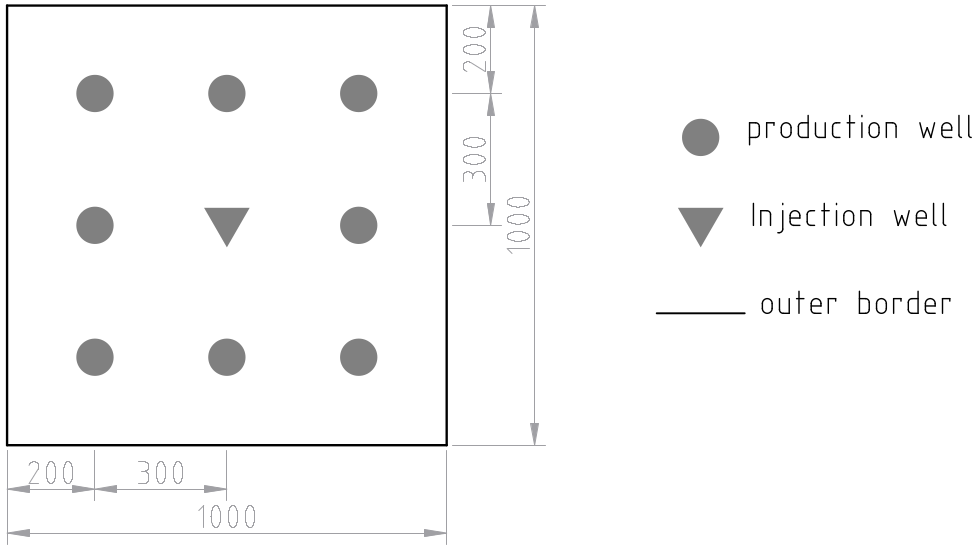
\includegraphics[height=12pc]{fig1.png}}
    \caption{Схематическое представление расчётной области.}
	\label{fig:map}
\end{figure}

Месторождение разрабатывается при помощи 8 добывающих и 1 нагнетательной скважины. Период разработки составляет 30 лет, контур питания был “подключён” по периметру расчетной области. Для решения задачи параметрической идентификации период разработки был разбит на 2 интервала: 20, 10 лет, соответственно:
\begin{enumerate}
\item с 01-2000 по 12-2005  интервал адаптации;
\item с 01-2006 по 12-2007  интервал валидации;
\item с 01-2008 по 12-2009  интервал прогноза.
\end{enumerate}

На интервале адаптации решается обратная задача для всех 4-х моделей, находятся неизвестные параметры. На интервале валидации оцениваются прогнозные характеристики настроенной модели, и осуществляется выбор модели, обладающей наилучшими прогнозными характеристиками. Дополнительно был выделен 3-й интервал - интервал прогноза, на котором производится оценка поведения выбраной модели при значительном изменении управляющих параметров. Временной интервал для этапа адаптации выбирался таким образом, чтобы он включал в себя поэтапный ввод в эксплуотацию всех скважин и был достигнут стационарный режим эксплуотации. Этап валидации включает в себя период стационарной работы месторождения. 

Для этапа прогнозирования было рассчитано 3 сценария эксплуатации для каждой модели, и произведено сопоставление поведение основных параметров разработки. В качестве сценариев были расчитаны: S0 - стационарный режим работы при котором не меняется объём нагнетаемой жидкости, S1 - двукратное сокращение объёма нагнетаемой жидкости и S2 - двукратное увеличение объёма нагнетаемой жидкости по сравнению со сценарием S0. 

На рисунке \ref{fig:din} представлена динамика среднего пластового давления для фактических данных (B - базовый вариант) и моделей водоносного горизонта (M1-M4 модели аквифера). На рисунке \ref{fig:hist} ввиде гистограммы показанны значения целевой функции (\ref{mape}) для интервалов адаптации (adp) и валидации (val), которая характеризует отличие вариантов M1-M4 от варианта B.
\begin{figure} 
    \begin{minipage}[h]{0.48\linewidth}
      \center{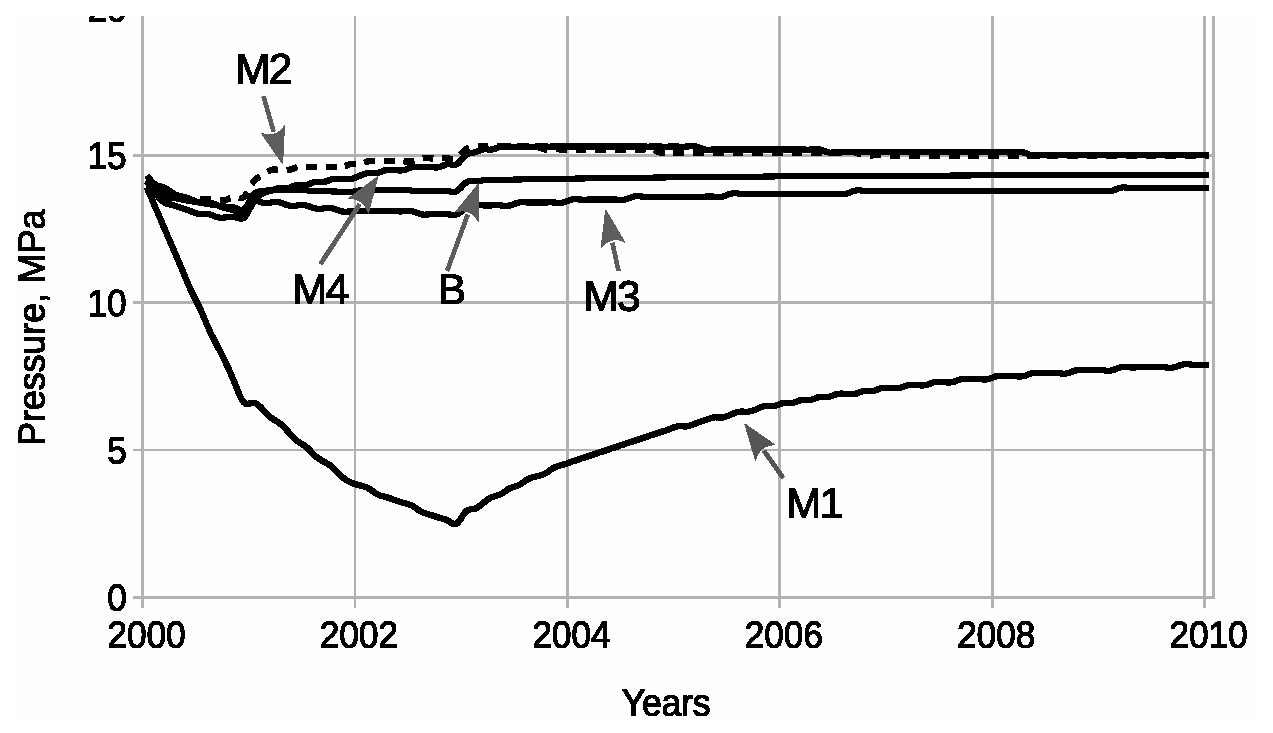
\includegraphics[height=0.60\linewidth]{fig2.eps}}
      \caption{Динамика среднего пластового давления при разных моделях водоносного горизонта}
      \label{fig:din}
    \end{minipage} \hfill
    \begin{minipage}[h]{0.48\linewidth}
      \center{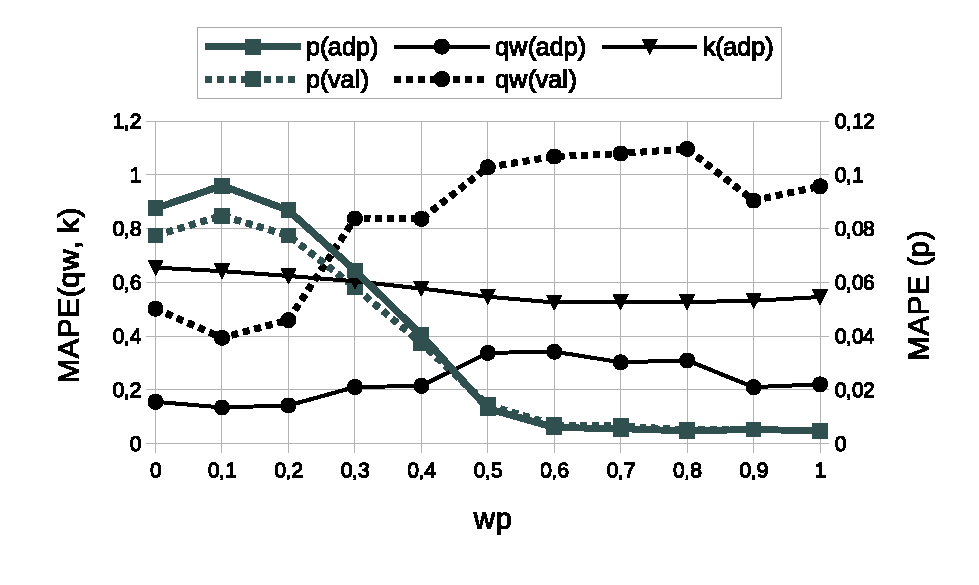
\includegraphics[height=0.60\linewidth]{fig3.eps}}
      \caption{Значения целевой функции для этапов адаптации (adp) и валидации (val)}
      \label{fig:hist}
    \end{minipage} 
\end{figure}
Из рисунков видно, что модель M1 обладает наихудшими показателями как на этапе адаптации так и на этапе валидации. Значение целевой функции примерно на порядок больше, чем у остальных моделей, следовательно, модель М1 наименне пригодня для описания поведения моделируемого объета и в дальнейших исследованиях она использоваться не будет. Наилучшими характеристиками для адаптации и валидации обладает модель M3. Модели M2 и M4 имею удовлетворительные значения целевой функции. Если сравнивать только две эти модели, то M4 лучше описывает историю, а M2 - имеет лучшие прогнозные свойства, соответсвенно выбор из этих двух моделей необходимо осуществлять используюя некоторые другие критерии например такие как BIC (\cite{mus}).

На практие, как правило, решеется только задача адаптации, и выбор модели осуществляется экспертно. Отбраковка моделей производится в основном по критерию не привышения ошибки, заложенной в различных регламентах (обычно от 5 до 25\%). Соотсветсвенно модели M2-M4 ввиду сравнительно малого отличия их показателей могут быть равновероятно выбраны в качестве прогнозирующих моделей. Действительно, наиболее ярко отличие динамики давления для разных моделей наблюдается в начальный период - при вводе новых скважин и выходе на стационарные режимы работы скважин. При стационарных режимах модели имеют близкие прогнозные характеристики. 

Интересным является поведение адаптированной модели при значительном (экстремальном) изменении режима работы скважин, реализованы в сценариях S1 и S2. На рисунке \ref{fig:2din} представлена динамика среднего пластового давления для трёх моделей (M2-M4) при трёх сценариях разработки (S0-S2).
\begin{figure}
\center{ 
    \begin{minipage}[h]{0.32\linewidth}
      \center{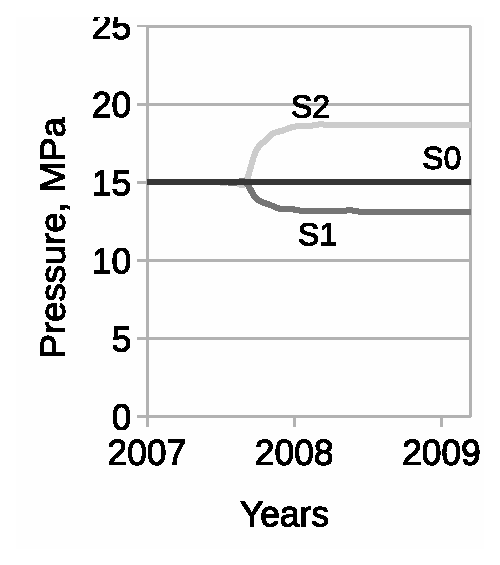
\includegraphics[height=0.92\linewidth]{fig4a.eps} \\ (a)}
    \end{minipage} \hspace{0pt}
    \begin{minipage}[h]{0.32\linewidth}
      \center{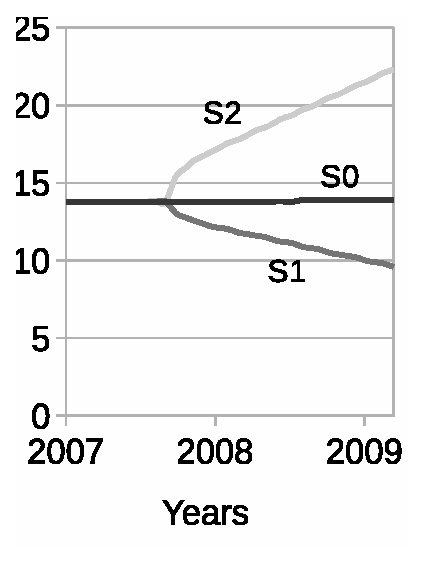
\includegraphics[height=0.92\linewidth]{fig4b.eps} \\ (b)}
    \end{minipage} \hspace{0pt}
    \begin{minipage}[h]{0.32\linewidth}
      \center{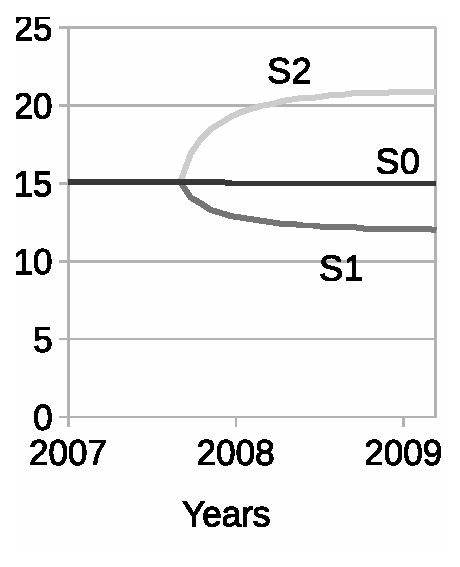
\includegraphics[height=0.92\linewidth]{fig4c.eps} \\ (c)}
    \end{minipage} 
    \caption{Динамика среднего пластового давления для 3-х моделей водоносного горизонта при 3-х сценариях разработки, где a, b и c соответствуют M2, M3 и M4.}
    \label{fig:2din}
    }
\end{figure}
Как видно из графиков, поведение кривых давления при одинаковых сценариях (S1 и S2) для разных моделей различны. Отличие заключается не только в значениях пластового давления, но и в динамике его изменения. Соответственно прогнозные показатели каждой модели будут существенно отличаться. Для поддержания качетва прогнозных свойств модели в допустимых пределах в условиях существенных изменений режимов работы, процедура актуализации модели является необходимой.

\section{CONCLUSIONS}

В результате исследования было показано, что получить удовлетворительное решение обратной задачи можно используя модели различной степени сложности. Помимо качества настройки модели на историю разработки - качества адаптации, также необходимо оценивать её прогнозные свойства. Проведение процедуры валидации позволяет осуществить выбор модели, имеющей наилучшие прогнозные характеристики. Кроме того, в работе было продемонстрированно, что качество прогноза помимо, сложности модели, зависит от сценариев разработки на которых адаптировалась и валидировалась модель. При  значительном отличии прогнозируемых режимов от тех, на которых была осуществлена настройка модели, прогнозные свойства модели резко снижаются. По мере поступления фактических данных необходимо заново проводить процедуру структурно-параметрической идентификации.

\section{FUNDING}
The research was carried out within the framework of the Program of Fundamental Scientific Research of the state academies of sciences in 2013-2020 (project No. AAAA-A17-117030610130-1).

%
% The Bibliography
%
\begin{thebibliography}{99}
\bibitem{mus} E.N.Musakaev, S.P.Rodionov, D.Y.Legostaev, V.P.Kosyakov,  «Parameter identification for sector filtration model of an oil reservoir with complex structure» // AIP Conference Proceedings 2125,030113 2019;

\bibitem{kos} V.P.Kosyakov, D.Y.Legostaev,  «Computational technology for solution of the reverse problem of filtration theory for oil fields with an aquifer» // AIP Conference Proceedings 2125,030112 2019;

\bibitem{bas} К.С.Басниев, Н.М.Дмитриев, Р.Д.Каневская, В.М.Максимов. Подземная гидромеханика.  М.-Ижевск: Институт компьютерных исследований, 2006. 

\bibitem{dake} L.P.Dake, Fundamentals of Reservoir Engineering (Elsevier, Amsterdam, 1978).

\bibitem{fet} M.J.Fetkovich. A Simplifi ed approach to water infl ux calculations – Finite aquifer systems. J. Pet. Tech. July 1971, vol. 23, is. 7, pp. 814–828.

\bibitem{opt} V.P.Kosyakov, S.P.Rodionov "Optimal control of wells on the basis of two-phase filtration equations". Proceedings of MIPT. 2016. V. 8, N 3. P. 79–90.


\end{thebibliography}

\end{document}